In order to improve the performance of FCNs and complete objective segmentation of the complex sense by using the level set method, the level set with the deep prior method is proposed as shown in Fig. \ref{fig: Flow diagram}.
\begin{figure}[h]
    \centering
    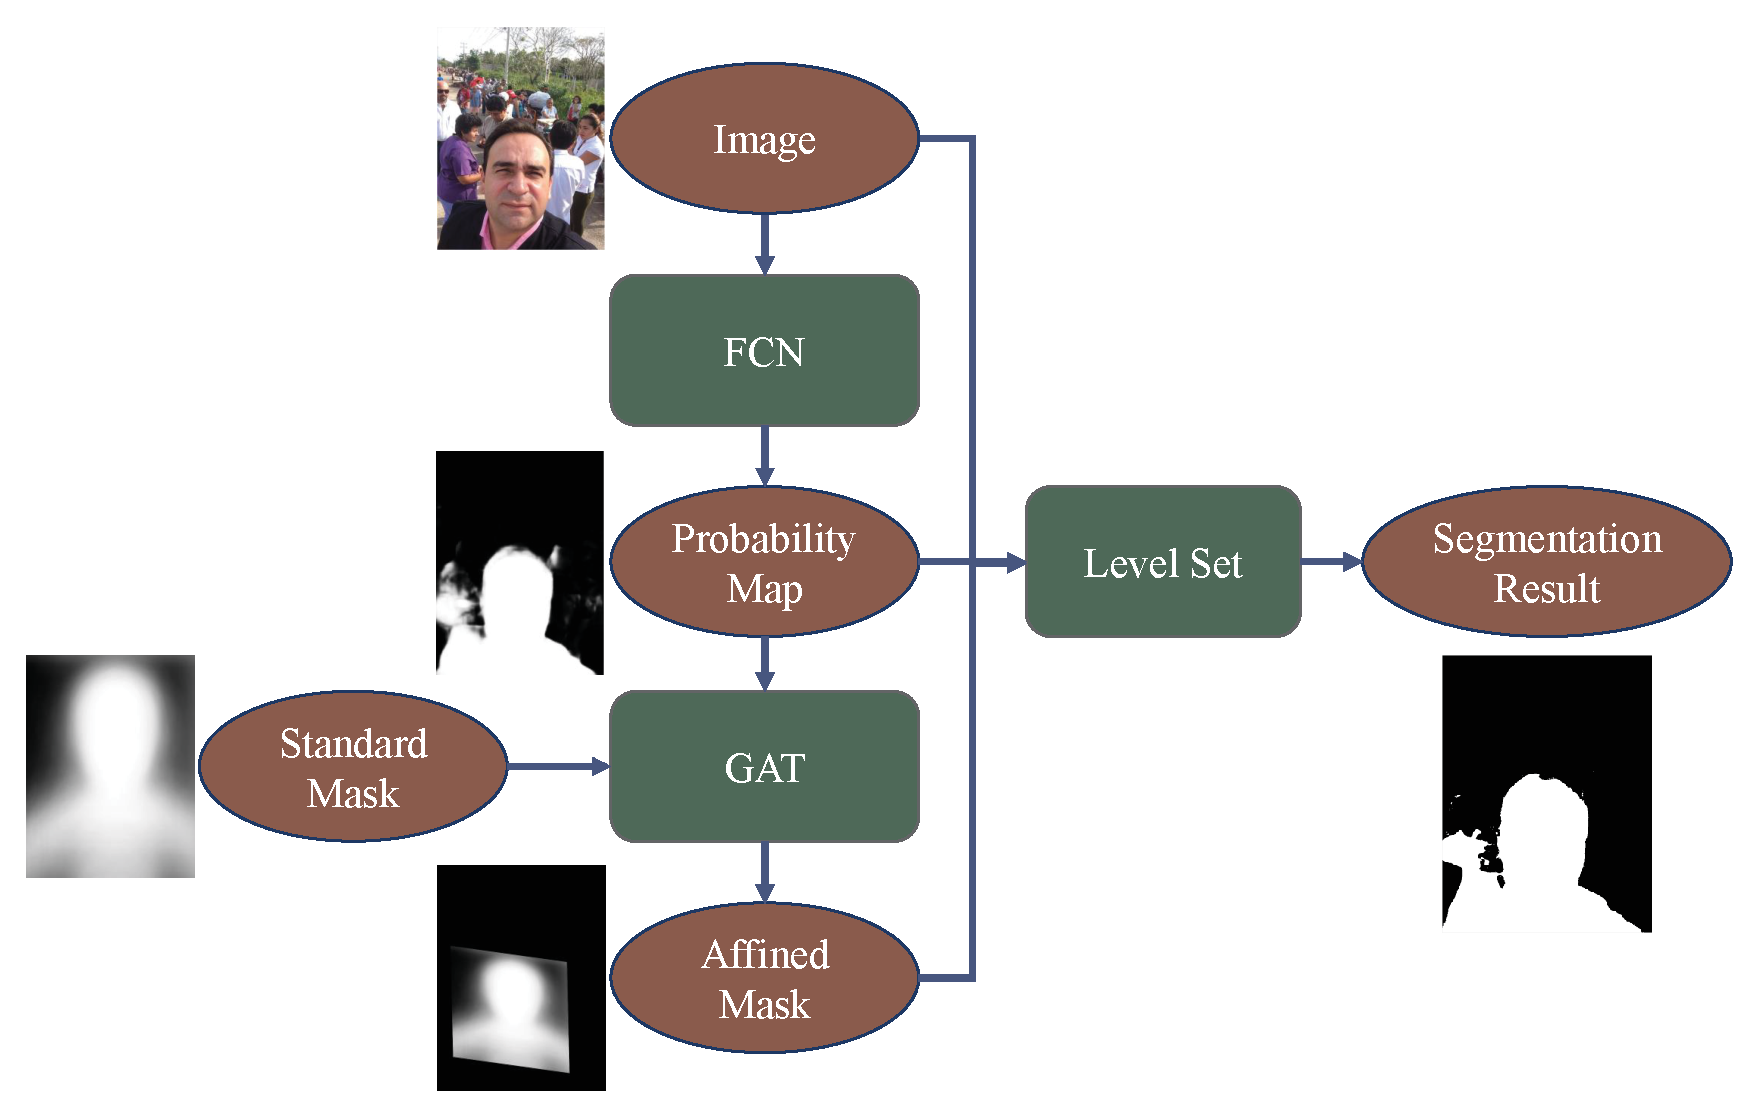
\includegraphics[width = 8cm]{figs/Flow_Diag.eps}
    \caption{The flow diagram of the proposed method.}\label{fig: Flow diagram}
\end{figure}
The output of FCNs is taken as a probability map that each pixel belongs to a different category. The segmentation shape represented by the probability map is noisy, but it still retains a large part of the correct segmentation. Therefore, an optimal affine transformation of the standard shape mask (the shape prior) of the image can be obtained based on the "probability" shape with the GAT method. Finally, the image, the probability map and the affine mask are used as the input of the level set method to implement the image segmentation.

\subsection{Deep Learning for the Probability Map}\label{subsec: FCNs for the Probability Map}
Deep Learning as an end-to-end method has achieved many excellent performances in semantic segmentation tasks. Because each pixel in the picture needs to be classified, the traditional network structure is useless. Long et al. proposed the FCN to replace the fully connected layer in the traditional convolution neural network (CNN) for classification into a convolution layer and realize the prediction of pixel-to-pixel \cite{FCN-original:long2015fully}. Then many semantic image segmentation frameworks based the FCN are used in different segmentation tasks. The structure of the FCNs is shown in Fig. \ref{fig: The structure of FCNs}.
\begin{figure*}[ht]
    \centering
    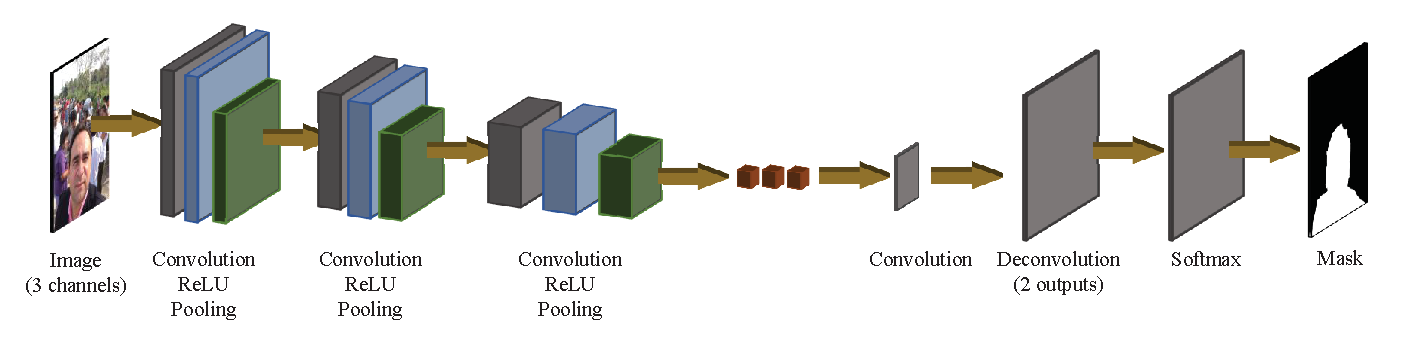
\includegraphics[width = 15cm]{figs/FCN.eps}
    \caption{The structure of FCNs.}\label{fig: The structure of FCNs}
\end{figure*}
There are several different types of layers in FCNs.
\paragraph*{Convolution Layer}
The convolution is often used to detect features in a picture. And many convolution-based feature extraction operators are proposed, such as edge detection \cite{Convolution:edge:canny1987computational} and corner detection \cite{Convolution:corner:harris1988combined}. Unlike traditional convolution kernels that are pre-designed, convolution kernels in CNNs are learnable and iteratively updated by the Back Propagation (BP) algorithm based on the training set. In terms of weights sharing, each feature map shares a convolution kernel. And in terms of the feature extraction, each convolution kernel extracts a pattern in each corresponding feature map of the previous layer. Therefore, the layered convolution structure makes the CNN having powerful feature extraction capabilities. As a result, many feature-based methods have been proposed to improve the CNN performance by improving the convolution kernel \cite{CNN:kernel:zhou2017oriented} or the network architecture \cite{CNN:arch:he2016deep}.

\paragraph*{ReLU Layer}
The ReLU is just a no-linear activation function: $f(x) = \max(0,x)$. This activation function can be regarded as a threshold function. And the output of irrelevant nodes is suppressed to obtain a sparse output.
\paragraph*{Pooling Layer}
The Pooling layer represents multiple adjacent points in the feature map as a single point by using the maximum or the mean method to greatly reduce the size of the feature map. However, due to the transitivity of features in the network structure of the CNN \cite{CNN:pooling:zhou2016learning}, a point in a small feature map represents a large number of points in the original picture, which makes the information be dispersed in different small feature maps. Meanwhile, the information of location and shape details in the picture are weakened. Because, the image has the characteristics of pixel aggregation and the image information can be expressed in a compressed manner, the Pooling layer is effective in the CNN.
\paragraph*{Deconvolution Layer}
The Deconvolution layer is used to restore the size of the feature map reduced by the Pooling layer, making them the same size as the original image. It implements a learnable upsampling process by transposing the convolution kernels \cite{CNN:deconvolution:zeiler2011adaptive}.
\paragraph*{Softmax Layer}
The Softmax Layer converts the output of the FCN to a form of probability through the softmax function as shown in Eq. (\ref{eq: Softmax}).
\begin{equation}\label{eq: Softmax}
    p_{x,y}(c=i) = \frac{\exp(h_i(x,y))}{\sum_j \exp(h_j(x,y))}
\end{equation}
where, $h_i(x,y)$ represents the value of the $i$-th feature map of the final output of FCN at the position $(x,y)$, and $p_{x,y}(c=i)$ represents the probability of the pixel at $(x,y)$ belonging to category $c=i$. In this paper, the output of the softmax layer is treated as a probability map to represent the probability of each pixel.

From the perspective of probability, the FCN is equivalent to a probability estimator, which is used to estimate the probability of category of the pixel at $(x,y)$. The probability of an image $I$ is expressed by Eq. (\ref{eq: probability expression}).
\begin{equation}\label{eq: probability expression}
    p_{x,y}(c=i \mid I)
\end{equation}
The distribution is a multinomial distribution with the experiment number $1$, so the probability $O_{x,y}(c)$ of category of the ground truth at each pixel $(x,y)$ is $1$. the value of $O_{x,y}(c)$ is $1$ when $c$ is the true category, or the value is $0$. Therefore, the minimizing cross entropy method is used to minimize the difference between the estimated probability and the true probability to train the FCN \cite{CNN:kingma2013auto}. And then the loss function is calculated through Eq. (\ref{eq: Multinoimal loss}).
\begin{equation}\label{eq: Multinoimal loss}
  \mathcal{L} = \sum_{x,y} \sum_{i}p_{x,y}(c=i\mid I)\log O_{x,y}(c=i\mid I)
\end{equation}
At the point of receptive fields \cite{CNN:hubel1962receptive}, the output of the FCN at each location in the picture is only related to the receptive field of this location. So the probability model above can be expressed as $p_{x,y}(c=i \mid \mathcal{R}_{x,y})$, and $\mathcal{R}_{x,y}$ represents the receptive field of output at $(x,y)$. Therefore, points with similar receptive fields will be predicted to the same category. Similarly, the similar regions in the original image are also predicted as the same category. But the output of the FCN is easily affected by the similar noise area.
\begin{figure}[ht]
    \centering
    \begin{minipage}[b]{2.5cm}
        \centering
        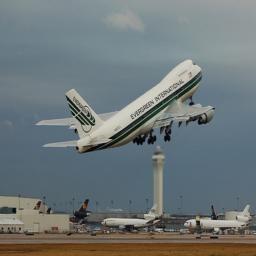
\includegraphics[width=2.5cm]{figs/Receptive_example_1_1.jpg}
        \caption*{a-1}
    \end{minipage}
    \mbox{\hspace{1cm}}
    \begin{minipage}[b]{2.5cm}
        \centering
        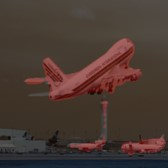
\includegraphics[width=2.5cm]{figs/Receptive_example_1_2.png}
        \caption*{a-2}
    \end{minipage}

    \begin{minipage}[b]{2.5cm}
        \centering
        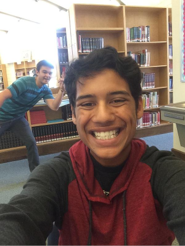
\includegraphics[width=2.5cm]{figs/Receptive_example_2_1.png}
        \caption*{b-1}
    \end{minipage}
    \mbox{\hspace{1cm}}
    \begin{minipage}[b]{2.5cm}
        \centering
        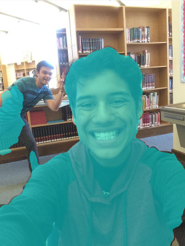
\includegraphics[width=2.5cm]{figs/Receptive_example_2_2.png}
        \caption*{b-2}
    \end{minipage}
    \caption{Some segmentation result of FCNs.}
    \label{fig: Recveptive Example}
\end{figure}
Some Segmentation results of FCNs are shown in Fig. \ref{fig: Recveptive Example} (The left is the original image and the right is the result of the segmentation by FCNs). The two pictures a-1 and a-2 in Fig. \ref{fig: Recveptive Example} are the example of the Pascal VOC data set, which is segmented by FCN8s \cite{FCN-original:long2015fully}. It can be seen that the white beacon in the center of the picture is incorrectly predicted as an aircraft. The two pictures b-1 and b-2 in Fig. \ref{fig: Recveptive Example} are from a portrait data set, and segmented by the PortraitFCN \cite{FCN:segmentation:shen2016automatic} which is the retraining of FCN8s in the Portrait data set.
From these two segmentation results, we can get some shortcomings of FCNs in segmentation tasks.
\begin{itemize}\label{itemize: FCN shortcomings}
  \item First, the segmentation boundary cannot be accurately adapted to the target boundary.
  \item Second, the segmentation boundary is rough and noisy.
  \item Finally, the prior information of the target shape is not considered.
\end{itemize}

Therefore, FCNs combined with Conditional Random Fields (CRF) \cite{FCN:CRF:zheng2015conditional} or Markov Random Field (MRF) \cite{FCN:MRF:liu2015semantic} are proposed to solve the first and second problems, and achieved a good performance. In order to solve the total three problems at the same time, the FCNs with level set method is proposed in this paper. After training on the training set, FCNs can extract features of the target and learn patterns of the target, and these capabilities are represented in the probability map. Therefore, the probability map preserves the information of the segmentation target based on the pixels in the receptive field. For example, in the Portrait data set, the probability map can represent the probability that each pixel belongs to a person. Although there is a certain probability which is incorrect, it still keeps most of the correct predictions, even the correct patterns information. Based on these properties of the probability map, it is possible to use the method of combining the probability map with the shape priors and the level set method for the semantic segmentation. And then how to get the optimal affine transformation of the standard shape prior using the GAT is introduced in the following subsection.

\subsection{Global Affine Transformation for Shape Prior Corrected}\label{subsec: Global Affine Transformation for Shape Prior Corrected}
There is only one mean mask of the portrait in the portrait data set \cite{FCN:segmentation:shen2016automatic}, which is called the standard shape prior in this paper as shown in Fig. \ref{fig: The standard shape mask}.
\begin{figure}[ht]
    \centering
    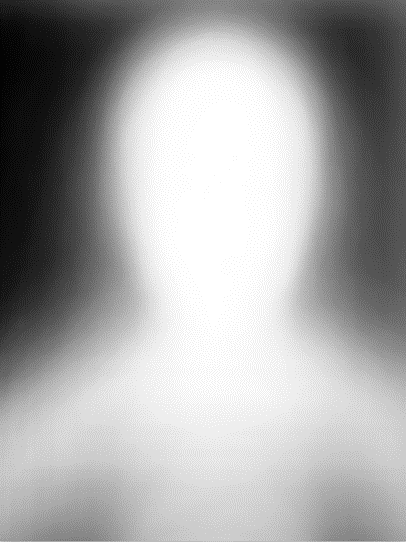
\includegraphics[width = 2.5cm]{figs/meanmask}
    \caption{The standard shape mask}\label{fig: The standard shape mask}
\end{figure}
In this subsection, the standard shape prior is transformed to the best position of the picture, based on the probability map obtained in the previous subsection. The transformation is assumed as the affine transformation which only contains translation, scale, rotation, flip and shear, and does not change the basic geometry of the original shape. Since the probability map is similar to the real shape, and the optimal affine transformation of the standard shape prior can be obtained based on the probability map.

The GAT is used to obtain the optimal affine transformation. The GAT was first used to find the optimal affine transformation between handwritten characters \cite{GAT:wakahara1998adaptive} \cite{GAT:xiaona2007hierarchical}. It accepts a set of contour coordinates of the shape, so the probability map and the standard shape need to be converted to contours. The sample contour of the probability map and the standard shape prior is shown in Fig. \ref{fig: The sample contour of the probability map and standard shape prior}.
\begin{figure}[h]
    \centering
    \begin{minipage}[b]{2cm}
        \centering
        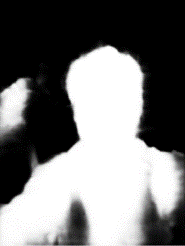
\includegraphics[width=2cm]{figs/GAT_Contour_1_1.png}
        \caption*{a-1}
    \end{minipage}
    \mbox{\hspace{1cm}}
    \begin{minipage}[b]{2cm}
        \centering
        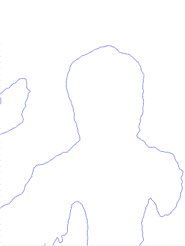
\includegraphics[width=2cm]{figs/GAT_Contour_1_2.png}
        \caption*{a-2}
    \end{minipage}

    \begin{minipage}[b]{2cm}
        \centering
        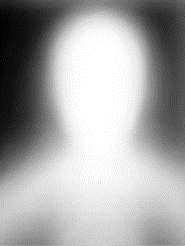
\includegraphics[width=2cm]{figs/GAT_Contour_2_1.png}
        \caption*{b-1}
    \end{minipage}
    \mbox{\hspace{1cm}}
    \begin{minipage}[b]{2cm}
        \centering
        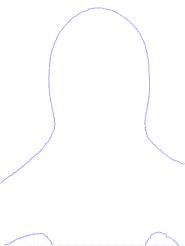
\includegraphics[width=2cm]{figs/GAT_Contour_2_2.png}
        \caption*{b-2}
    \end{minipage}
    \caption{The sample contour of the probability map (a-1, a-2 of Fig. \ref{fig: Recveptive Example}. b-1) and standard shape prior (b-1, b-2).}
    \label{fig: The sample contour of the probability map and standard shape prior}
\end{figure}
Let the original (probability map) contour set is $S$ and the target (standard shape prior) contour set is $R$:
\begin{eqnarray*}
% \nonumber to remove numbering (before each equation)
  S &=& \{s_1, s_2, \cdots, s_i, \cdots, s_m \} \\
  R &=& \{r_1, r_2, \cdots, r_j, \cdots, r_n\}
\end{eqnarray*}
where $s_i$ is the coordinate vector of the $i$-th point of contour $S$ and $r_j$ is the coordinate vector of the $j$-th point of contour $R$. $s_i$ can be transformed into a new coordinate vector $\hat{s}_i$ by a affine transformation:
\begin{equation}
    \hat{s}_i = A s_i + b
\end{equation}
where $A$ is a $2\times 2$ matrix, and $b$ is a $2\times 1$ vector. The transformed contour is represented by $\hat{S}$.
\begin{equation*}
    \hat{S} = \{\hat{s}_1, \hat{s}_2, \cdots, \hat{s}_i, \cdots, \hat{s}_m\}
\end{equation*}
In order to get the optimal transformation, the distance between $S$ and $\hat{S}$ is minimized, and the distance $\mathcal{D}$ is defined as follows:
\begin{equation}\label{eq: Distance of GAT}
\mathcal{D} = \frac{1}{2}\left[ \frac{1}{m}\sum_i^m \underset{j}{\min}\left\|\hat{s}_i - r_j\right\|^2 + \frac{1}{n}\sum_j^n \underset{i}{\min}\left\|\hat{s}_i-r_j\right\|^2 \right]
\end{equation}
Based on $A$ and $b$, the distance $\mathcal{D}$ is minimized.
\begin{equation}\label{eq: Argmin of GAT}
    A,b = \underset{A,b}{\arg\min} \ \ \mathcal{D}
\end{equation}
There are two $\min$ operations in Eq. (\ref{eq: Distance of GAT}), so $A$ and $b$ cannot be directly calculated by Eq. (\ref{eq: Argmin of GAT}). A computable model based on weighted least-squares criterion is proposed to solve this combinatorial optimization problem \cite{GAT:wakahara1998adaptive}. The objective function $\Phi$ is defined as
\begin{multline}\label{eq: new objective funtion of GAT}
    \Phi = \frac{1}{2}\left[ \frac{1}{m}\sum_i^m\sum_j^n \mu_{ij}(D)\left\|\hat{s}_i-r_j\right\|^2 \right. \\
    \left. + \frac{1}{n}\sum_j^n\sum_i^m \nu_{ji}(D)\left\|\hat{s}_i-r_j\right\|^2 \right]
\end{multline}
\begin{align*}
% \nonumber to remove numbering (before each equation)
  \mu_{ij}(D) &= \exp\left[-\frac{\left\|s_i-r_j\right\|^2 - \underset{k}{\min}\left\| s_i-r_k \right\|^2}{D} \right] \\
  \nu_{ji}(D) &= \exp\left[-\frac{\left\|s_i-r_j\right\|^2 - \underset{k}{\min}\left\| s_k-r_j \right\|^2}{D} \right]
\end{align*}
\begin{equation}\label{eq: global of GAT}
    D = \frac{1}{2}\left[ \frac{1}{m}\sum_i^m\underset{j}{\min}\left\| s_i-r_j \right\|^2 + \frac{1}{n}\sum_j^n\underset{i}{\min}\left\| s_i-r_j \right\|^2 \right]
\end{equation}
The $\min$ operation is replaced with weighted summations using Gaussian functions of $\mu_{ij}(D)$ and $\nu_{ji}(D)$. The shortest distance between all points in $S$ and $R$ is considered in Eq. (\ref{eq: global of GAT}), so this method is called the "Global" Affine Transformation. And Eq. (\ref{eq: global of GAT}) can be rewritten as follows,
\begin{equation}
    \Phi = \frac{1}{2} \sum_i^m\sum_j^n \rho_{ij}(D)\left\| \hat{s}_i - r_j \right\|^2
\end{equation}
\begin{equation*}
    \rho_{ij}(D) = \frac{\mu_{ij}(D)}{m} + \frac{\nu_{ji}(D)}{n}
\end{equation*}
Thus, the minimization of distance $\Phi$ can be obtained by solving the following equations:
\begin{equation}\label{eq: equations of GAT}
    \left\{\begin{matrix}
        \frac{\partial \Phi}{\partial A} =& \sum_i^m\sum_j^n\rho_{ij}(D)s_i(As_i+b-r_j)^T &= 0 \\
        \frac{\partial \Phi}{\partial b} =& \sum_i^m\sum_j^n\rho_{ij}(D)(As_i+b-r_j) &= 0 \\
    \end{matrix}\right.
\end{equation}
Gaussian elimination can be used to solve Eq. (\ref{eq: equations of GAT}), and there are $6$ unknown parameters in total. The GAT is used to find the optimal transformation within the neighborhoods of each point, so the final optimal affine transformation can be obtained through iterative methods, and the detailed proof is given by Toru Wakahara \cite{GAT:wakahara1998adaptive}.

Every point in contour $S$ is disposed by the above affine transformation, and the optimal affine transformation can also be applied in the image \cite{GAT:CV:hartley2003multiple}. And the transformation matrix is defined as follows:
\begin{equation*}
    T = \begin{bmatrix}
          A_{1,1} & A_{2,1} & 0 \\
          A_{1,2} & A_{2,2} & 0 \\
          b_1 & b_2 & 1 \\
        \end{bmatrix}
\end{equation*}
Then, the transformation $T$ can be applied in the standard shape prior image with interpolation to get the shape prior corrected. Some results of the GAT in Portrait data set are shown in Fig. \ref{fig: Some results of the GAT}.
\begin{figure}[h]
    \centering
    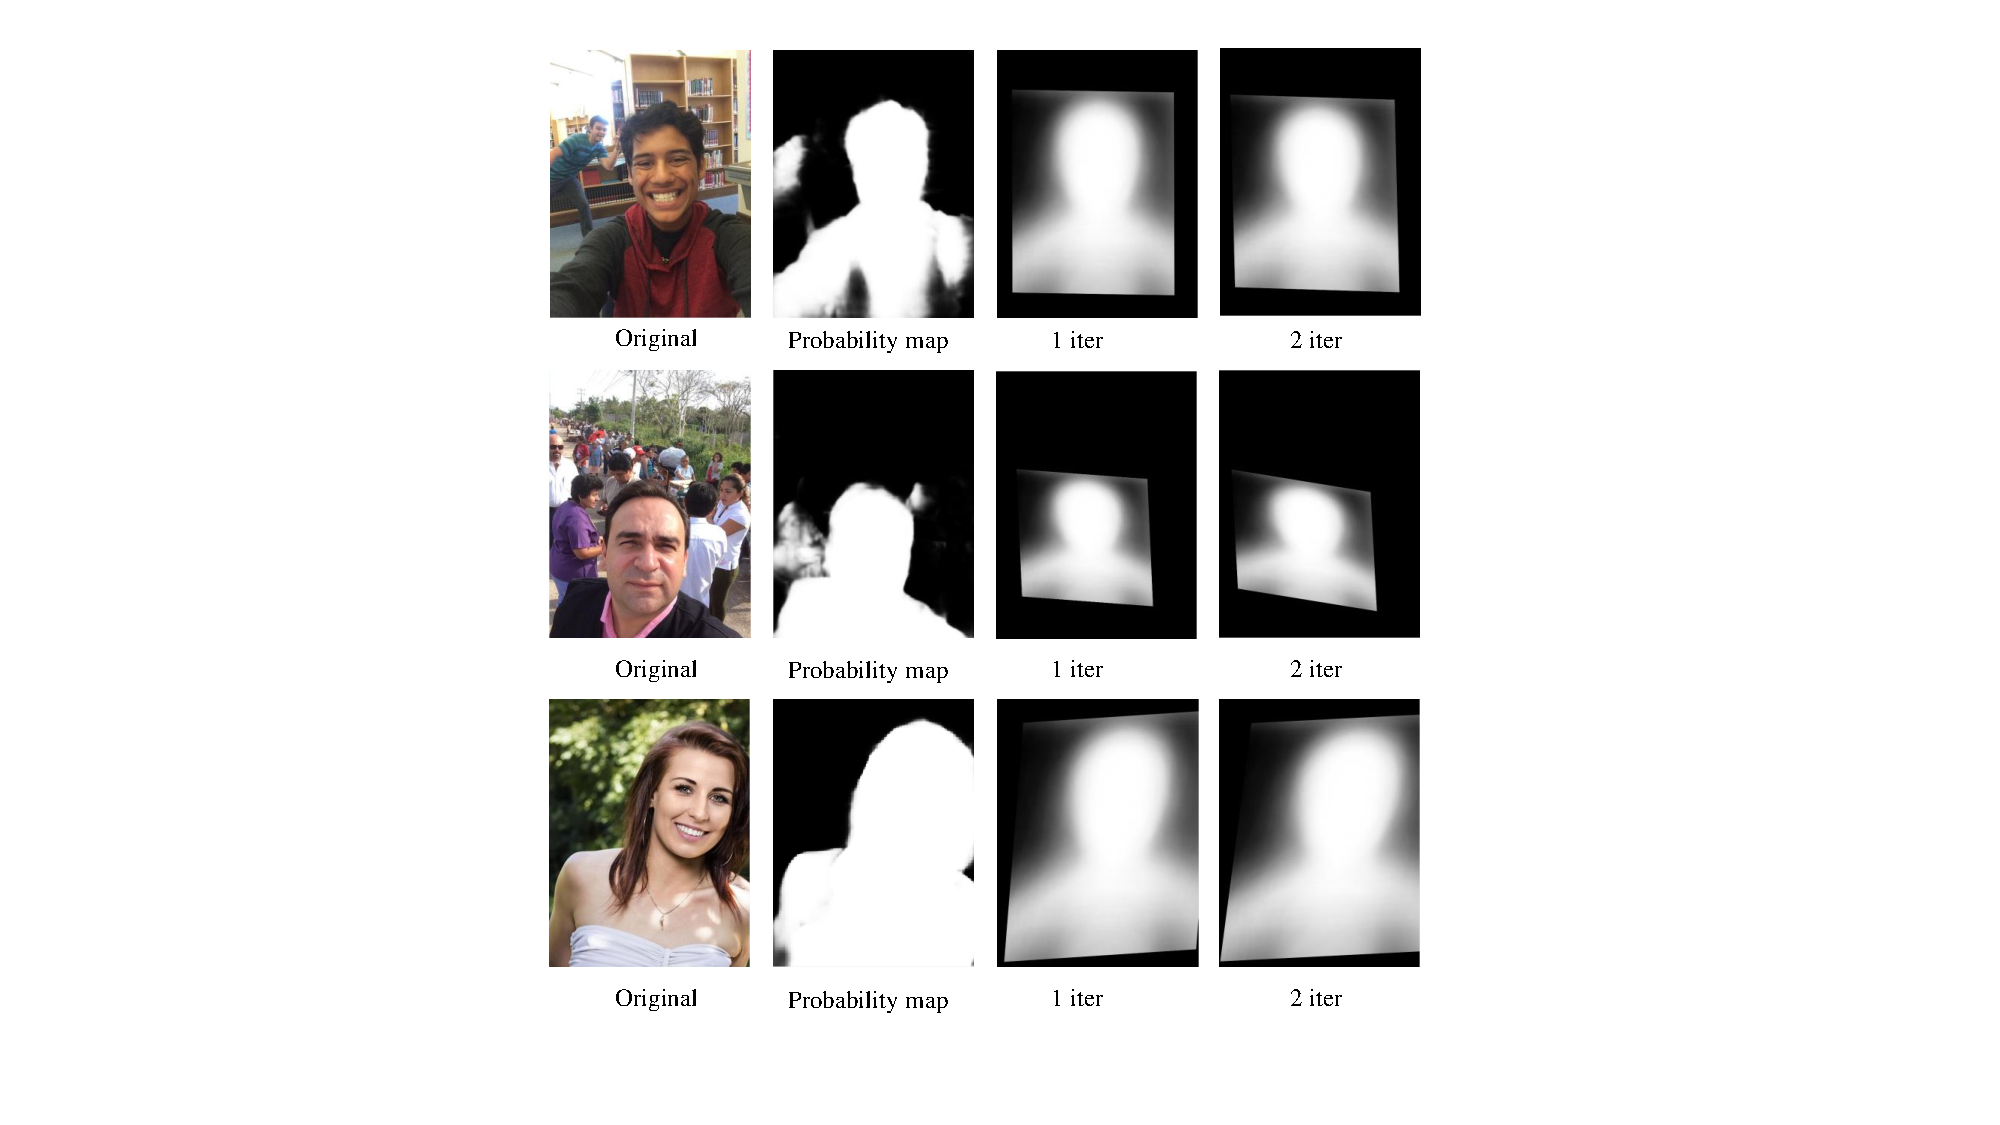
\includegraphics[width=8cm]{figs/GAT_Result.eps}
    \caption{Some results of the GAT in Portrait data set.}
    \label{fig: Some results of the GAT}
\end{figure}
From Fig. \ref{fig: Some results of the GAT}, we can see that even if the probability map is noisy, the GAT can still fit the shape expressed by the probability map. And the transformed shape prior shape is already very close to the shape of the probability map at $1$ iter, so the GAT is effective.

\subsection{Level Set with Deep Prior Method for Image Segmentation}\label{subsec: Level Set Method for Image Segmentation}
The level set method for the image segmentation is a region-based active contour model, which is a variational method based on the energy minimization to evolve the level set \cite{LevelSet:malladi1995shape}. The level set is denoted by $\phi$ and the zero level $\phi=0$ is regarded as the contour of target, and the region of $\phi<0$ is regarded as the target region. The level set $\phi$ can be viewed as a potential function that represents the strength of each point in the image. Therefore, the level set $\phi$ can be treated as a kind of probability density, indicating the probability met by the point \cite{LevelSet:prob:cremers2008shape}. Moreover, the energy objective function of the level set method can be combined with many energy-based probability models to expand its capabilities \cite{LevelSet:prob:chen2013deep}.

The most classic level set method is the \emph{CV} model proposed by Chan and Vese \cite{LevelSet:chan2001active}, and the energy function of the contour is obtained by Eq. (\ref{eq: Level Set CV contour energy function}).
\begin{equation}\label{eq: Level Set CV contour energy function}
\begin{split}
    \mathcal{F}(C,c1,c2) = & \lambda_1\int_{\text{outside}(C)}\left|I(\mathbf{x})-c_1\right|^2 \mathrm{d}\mathbf{x} \\
     & + \lambda_2\int_{\text{inside}(C)}\left| I(\mathbf{x}) - c_2 \right|^2 \mathrm{d}\mathbf{x} \\
     & + \nu\left| C \right|
\end{split}
\end{equation}
where $\text{outside}(C)$ and $\text{inside}(C)$ represent the regions outside and inside the contour $C$, respectively. $\mathbf{x}$ is a 2 dim vector that represents the image. $|C|$ represents length of the contour $C$. $c_1$ and $c_2$ are the statistics of the pixels outside and inside the contour, respectively. The energy function can be rewritten as the form of the level set function $\phi$:
\begin{equation}\label{eq: Level Set CV phi energy function}
    \begin{split}
        \mathcal{F}(\phi, c_1, c_2) =
        & \lambda_1 \int \left| I(\mathbf{x}) - c_1 \right|^2 H(\phi) \mathrm{d}\mathbf{x} \\
        & + \lambda_2 \int \left| I(\mathbf{x}) - c_2 \right|^2 (1-H(\phi)) \mathrm{d}\mathbf{x} \\
        & + \nu \int \left| \nabla H(\phi) \right| \mathrm{d}\mathbf{x}
    \end{split}
\end{equation}
where $H(z)$ is Heaviside function that indicates the regions of outside and inside represented by the level set function.
\begin{equation}
    H(z) = \left\{
            \begin{matrix}
             1, & z\geq 0 \\
             0, & z < 0 \\
            \end{matrix}\right.
\end{equation}
In order to introduce energy-based variational methods, the function $H$ is smoothed to make it possible to get gradients.
\begin{equation}\label{eq: equation epsilon}
  H_\epsilon(z) = \frac{1}{2}\left[ 1+\frac{2}{\pi}\arctan\left(\frac{z}{\epsilon}\right) \right] \\
\end{equation}
So the derivative of $H$ can be approximated by the derivative of $H_\epsilon$ based on Eq. (\ref{eq: H derivative}).
\begin{equation}\label{eq: H derivative}
  \delta_\epsilon(z) = H'_\epsilon(z) = \frac{1}{\pi}\frac{\epsilon}{\epsilon^2 + z^2}
\end{equation}
And the curves of $H$ and $\delta$ functions of different $\epsilon$ are shown in Fig. \ref{fig: The function figures of different epsilon}.
\begin{figure}[h]
    \centering
    \begin{minipage}[b]{4cm}
        \centering
        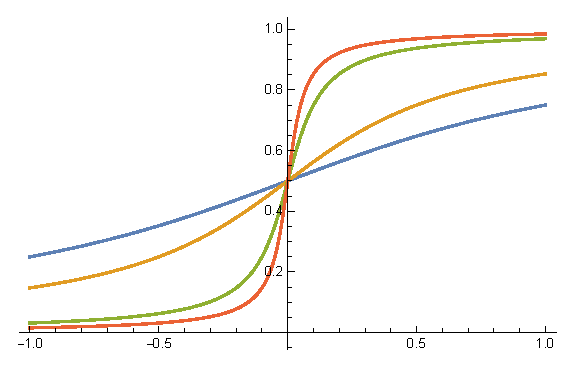
\includegraphics[width=4cm]{figs/H.eps}
        \caption*{$H_\epsilon(z)$}
    \end{minipage}
    \mbox{\hspace{0.2cm}}
    \begin{minipage}[b]{4cm}
        \centering
        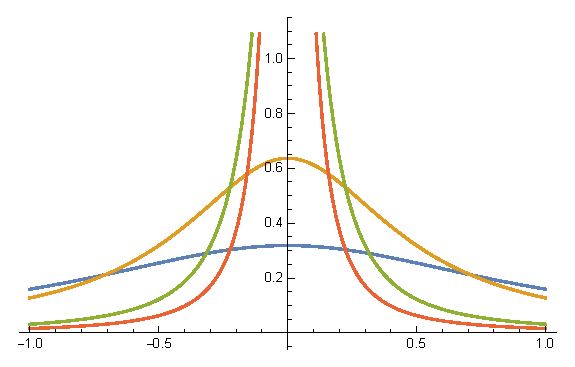
\includegraphics[width=4cm]{figs/delta.eps}
        \caption*{$\delta_\epsilon(z)$}
    \end{minipage}
    \caption{The function figures of different $\epsilon \in \{1, 0.5, 0.1, 0.05\}$.}
    \label{fig: The function figures of different epsilon}
\end{figure}

The level set method has a very flexible definition of the energy function, so it can be convenient to combine the original image, the probability map and the corrected shape prior information into an energy function. The energy function is defined as the following.
\begin{equation}\label{eq: All energy function of Level Set}
    \mathcal{F}(\phi) = \mathcal{E}_{\text{img}} + \mathcal{E}_{\text{shape}} + \mathcal{E}_{\text{edge}} + \mathcal{E}_{\text{reg}}
\end{equation}

All the items in Eq. (\ref{eq: All energy function of Level Set}) will be described in detail as follows.

\subsubsection{$\mathcal{E}_{\text{img}}$}
The first item refers to a improved \emph{CV} model proposed by Li \cite{LevelSet:mathod:li2008minimization}, which introduces a weight function. And each point uses the weighted statistics of its neighbors as a reference value. And the probability map is added in this item, $\mathcal{E}_{\text{img}}$ is defined as
\begin{equation}\label{eq: E_img of Level Set}
\begin{split}
    \mathcal{E}_{\text{img}} = &\sum_{i=1}^2 \lambda_i\int P_i(\mathbf{x}) \\
    & \cdot \left( \int K_\sigma(\mathbf{x}-\mathbf{y})\left| I(\mathbf{y}) - f_i(\mathbf{x}) \right|^2 M_i(\phi(\mathbf{y}))\mathrm{d}\mathbf{y} \right)\mathrm{d}\mathbf{x}
\end{split}
\end{equation}
where $P_1(\mathbf{x})$ and $P_2(\mathbf{x})$ are probability maps and represent the probability of background and target at point $\mathbf{x}$, respectively. $M_1(\phi) = H(\phi)$ and $M_2(\phi) = 1-H(\phi)$ represent the regions of outside and inside contour $C$, respectively. $K(u)$ represents a symmetrical weighted function and is used to weight neighbors of each point. The Gaussian kernel is often chosen as the weighted function,
\begin{equation}\label{eq: gaussian sigma}
    K_\sigma(u) = \frac{1}{\sigma\sqrt{2\pi}}e^{-\frac{|u|^2}{2\sigma^2}}
\end{equation}
$f_1(\mathbf{x})$ and $f_2(\mathbf{x})$ represent the weighted statics at point $\mathbf{x}$ of outside and inside. In the iterative process of each step, it is necessary to fix $\phi$ first, and get $f_i$ at this time. Fix $\phi$, $f_i(\mathbf{x})$ can be obtained by minimizing the functional $\mathcal{E}_{\text{img}}$ in Eq. (\ref{eq: E_img of Level Set}) based on the \emph{Euler} equation.
\begin{equation}\label{eq: f_i of Level Set}
    f_i(\mathbf{x}) = \frac{\int K_\sigma(\mathbf{x}-\mathbf{y})M_i(\phi(\mathbf{y}))I(\mathbf{y})\mathrm{d}\mathbf{y}}
    {\int K_\sigma(\mathbf{x}-\mathbf{y})M_i(\phi(\mathbf{y}))\mathrm{d}\mathbf{y}}
\end{equation}
Since the integral can be converted into the convolution. And Eq. (\ref{eq: f_i of Level Set}) can be written as
\begin{equation}
    f_i(\mathbf{x}) =
    \frac{K_\sigma \ast \left[ M_i^\epsilon(\phi(\mathbf{x})) I(\mathbf{x}) \right] }
    {K_\sigma \ast M_i^\epsilon(\phi(\mathbf{x}))}
\end{equation}
Then, fix $f_1$ and $f_2$, the partial derivative needs to minimize the energy functional $\mathcal{E}_{\text{img}}$.
\begin{multline}\label{eq: Level Set 1-item}
    \frac{\partial \mathcal{E}_{\text{img}}}{\partial \phi} = \delta_\epsilon(\phi)\left(\lambda_1P_1e_1-  \lambda_2P_2e_2 \right) \\
    e_i(\mathbf{x}) = \int K_\sigma(\mathbf{y}-\mathbf{x})\left| I(\mathbf{x})-f_i(\mathbf{y}) \right|^2 \mathrm{d}\mathbf{y}
\end{multline}
Similarly, $e_i$ can also be converted into the convolution, and the Eq. (\ref{eq: Level Set 1-item}) needs to be expanded as the following:
\begin{equation}
    \begin{split}
        e_i(\mathbf{x}) =
        & I^2(\mathbf{x})\cdot\left[ K_\sigma(\mathbf{x})\ast \mathbf{1} \right] \\
        & - 2I(\mathbf{x})\cdot\left[ K_\sigma(\mathbf{x})\ast f_i(\mathbf{x}) \right] \\
        & + K_\sigma(\mathbf{x}) \ast f_i^2(\mathbf{x})
    \end{split}
\end{equation}
where $\mathbf{1}$ is a all-$1$ matrix. Since the interval $[-2\sigma, 2\sigma]$ already contains more than $95\%$ in the Gaussian kernel function, and the size of convolution kernel of $K_\sigma$ can be set to $4\sigma +1$.

\subsubsection{$\mathcal{E}_{\text{shape}}$}
The corrected shape prior guarantees that the final segmentation result is similar to the shape prior. And the energy function is defined as
\begin{equation}
    \mathcal{E}_{\text{shape}} = \sum_{i=1}^2 \pi_i \int S_i(\mathbf{x}) M_i(\phi(\mathbf{x})) \mathrm{d}\mathbf{x}
\end{equation}
where $S_1$ is the corrected shape prior, and $S_2 = 1- S_1$. The energy function is equivalent to calculate the difference between the segmentation shape and the prior shape. Minimizing $\mathcal{E}_{\text{shape}}$ makes the segmentation shape as close as possible to the prior shape, and the partial derivative is calculated by Eq. (\ref{eq: Level Set 2-item}).
\begin{equation}\label{eq: Level Set 2-item}
    \frac{\partial \mathcal{E}_{\text{shape}}}{\partial \phi} = \delta_\epsilon(\phi)(\pi_1 S_1 - \pi_2 S_2)
\end{equation}

\subsubsection{$\mathcal{E}_{\text{edge}}$}
As in Eq. (\ref{eq: Level Set CV phi energy function}), this functional energy is used to calculate the length of the segmentation contour, which ensures the segmentation contour is smooth.
\begin{align}
    \mathcal{E}_{\text{edge}}
    & = \nu \int \left| \nabla H_\epsilon(\phi(\mathbf{x})) \right|\mathrm{d}\mathbf{x} \nonumber \\
    & = \nu \int \delta_\epsilon(\phi)|\nabla\phi|\mathrm{d}\mathbf{x}
\end{align}
\begin{equation}\label{eq: Level Set 3-item}
    \frac{\partial \mathcal{E}_{\text{edge}}}{\partial \phi} = - \nu \delta_\epsilon(\phi)\nabla \times \frac{\nabla \phi}{|\nabla \phi|}
\end{equation}

\subsubsection{$\mathcal{E}_{\text{reg}}$}
This $\mathcal{E}_{\text{reg}}$ is obtained based on the \emph{Signed Distance Function}, which guarantees the basic shape of the level set method during the iterative process \cite{LevelSet:mathod:li2005level, LevelSet:mathod:li2010distance}.
\begin{equation*}
    \mathcal{E}_{\text{reg}} = \mu \int \frac{1}{2} \left( |\nabla\phi(\mathbf{x})| -1 \right)^2\mathrm{d}\mathbf{x}
\end{equation*}
\begin{equation}\label{eq: Level Set 4-item}
    \frac{\partial \mathcal{E}_{\text{reg}}}{\partial \phi} = -\mu\left\{ \nabla^2\phi - \nabla \times \frac{\nabla\phi}{|\nabla\phi|} \right\}
\end{equation}

Finally, the minimum energy functional $\mathcal{F}$ can be obtained though the steady state solution of the gradient flow equations with Eq. (\ref{eq: Level Set 1-item}), Eq. (\ref{eq: Level Set 2-item}), Eq. (\ref{eq: Level Set 3-item}) and Eq. (\ref{eq: Level Set 4-item}).
\begin{align}
    \frac{\partial \phi}{\partial t}
    & = -\frac{\partial \mathcal{F}}{\partial \phi} \nonumber \\
    & = -\left( \frac{\partial \mathcal{E}_{\text{img}}}{\partial \phi}
        + \frac{\partial \mathcal{E}_{\text{shape}}}{\partial \phi}
        + \frac{\partial \mathcal{E}_{\text{edge}}}{\partial \phi}
        + \frac{\partial \mathcal{E}_{\text{reg}}}{\partial \phi} \right)
\end{align}
The function $\phi$ is calculated iteratively.
\begin{equation} \label{eq: iter Level Set}
    \phi^t = \phi^{t-1} + \Delta t \cdot \frac{\partial \phi}{\partial t}
\end{equation}

The result of the contour evolution process of the proposed level set with the deep prior for the image segmentation is shown in Fig. \ref{fig: The contour evolution process of proposed Level Set method at Portrait data set}. The level set method has a flexible energy functional form, making it more convenient to integrate more useful information. This proposed level set with the deep prior method makes up their respective disadvantages of FCNs and the level set method.
